\documentclass[]{article}
\usepackage{lmodern}
\usepackage{amssymb,amsmath}
\usepackage{ifxetex,ifluatex}
\usepackage{fixltx2e} % provides \textsubscript
\ifnum 0\ifxetex 1\fi\ifluatex 1\fi=0 % if pdftex
  \usepackage[T1]{fontenc}
  \usepackage[utf8]{inputenc}
\else % if luatex or xelatex
  \ifxetex
    \usepackage{mathspec}
  \else
    \usepackage{fontspec}
  \fi
  \defaultfontfeatures{Ligatures=TeX,Scale=MatchLowercase}
\fi
% use upquote if available, for straight quotes in verbatim environments
\IfFileExists{upquote.sty}{\usepackage{upquote}}{}
% use microtype if available
\IfFileExists{microtype.sty}{%
\usepackage{microtype}
\UseMicrotypeSet[protrusion]{basicmath} % disable protrusion for tt fonts
}{}
\usepackage[margin=1in]{geometry}
\usepackage{hyperref}
\hypersetup{unicode=true,
            pdftitle={SWE Final Analyses},
            pdfborder={0 0 0},
            breaklinks=true}
\urlstyle{same}  % don't use monospace font for urls
\usepackage{graphicx,grffile}
\makeatletter
\def\maxwidth{\ifdim\Gin@nat@width>\linewidth\linewidth\else\Gin@nat@width\fi}
\def\maxheight{\ifdim\Gin@nat@height>\textheight\textheight\else\Gin@nat@height\fi}
\makeatother
% Scale images if necessary, so that they will not overflow the page
% margins by default, and it is still possible to overwrite the defaults
% using explicit options in \includegraphics[width, height, ...]{}
\setkeys{Gin}{width=\maxwidth,height=\maxheight,keepaspectratio}
\IfFileExists{parskip.sty}{%
\usepackage{parskip}
}{% else
\setlength{\parindent}{0pt}
\setlength{\parskip}{6pt plus 2pt minus 1pt}
}
\setlength{\emergencystretch}{3em}  % prevent overfull lines
\providecommand{\tightlist}{%
  \setlength{\itemsep}{0pt}\setlength{\parskip}{0pt}}
\setcounter{secnumdepth}{0}
% Redefines (sub)paragraphs to behave more like sections
\ifx\paragraph\undefined\else
\let\oldparagraph\paragraph
\renewcommand{\paragraph}[1]{\oldparagraph{#1}\mbox{}}
\fi
\ifx\subparagraph\undefined\else
\let\oldsubparagraph\subparagraph
\renewcommand{\subparagraph}[1]{\oldsubparagraph{#1}\mbox{}}
\fi

%%% Use protect on footnotes to avoid problems with footnotes in titles
\let\rmarkdownfootnote\footnote%
\def\footnote{\protect\rmarkdownfootnote}

%%% Change title format to be more compact
\usepackage{titling}

% Create subtitle command for use in maketitle
\providecommand{\subtitle}[1]{
  \posttitle{
    \begin{center}\large#1\end{center}
    }
}

\setlength{\droptitle}{-2em}

  \title{SWE Final Analyses}
    \pretitle{\vspace{\droptitle}\centering\huge}
  \posttitle{\par}
    \author{}
    \preauthor{}\postauthor{}
    \date{}
    \predate{}\postdate{}
  

\begin{document}
\maketitle

This R Markdown is a conglomerate of all the graphs created in SWE
analyses from SNODAS data collected from Climate Engine

\hypertarget{prelimary-analyses-from-data-below}{%
\subsubsection{Prelimary Analyses from data
below:}\label{prelimary-analyses-from-data-below}}

\begin{itemize}
\tightlist
\item
  Chuska recieves the most snow out of the three
\item
  2010 is a big anomaly at all three locations, was this a heavy
  precipitation year?
\item
  Black Mesa and Carrizo monthly means most closely correlated
\end{itemize}

\hypertarget{raw-daily-time-series}{%
\subsubsection{Raw daily time series}\label{raw-daily-time-series}}

\includegraphics{SWE_final_analyses_files/figure-latex/unnamed-chunk-3-1.pdf}

\hypertarget{monthly-mean-time-series}{%
\subsubsection{Monthly mean time
series}\label{monthly-mean-time-series}}

\includegraphics{SWE_final_analyses_files/figure-latex/unnamed-chunk-4-1.pdf}
\includegraphics{SWE_final_analyses_files/figure-latex/unnamed-chunk-4-2.pdf}

Black Mesa: red Chuska: blue Carrizo: green

\hypertarget{intra-monthly-anomalies}{%
\subsubsection{Intra Monthly Anomalies}\label{intra-monthly-anomalies}}

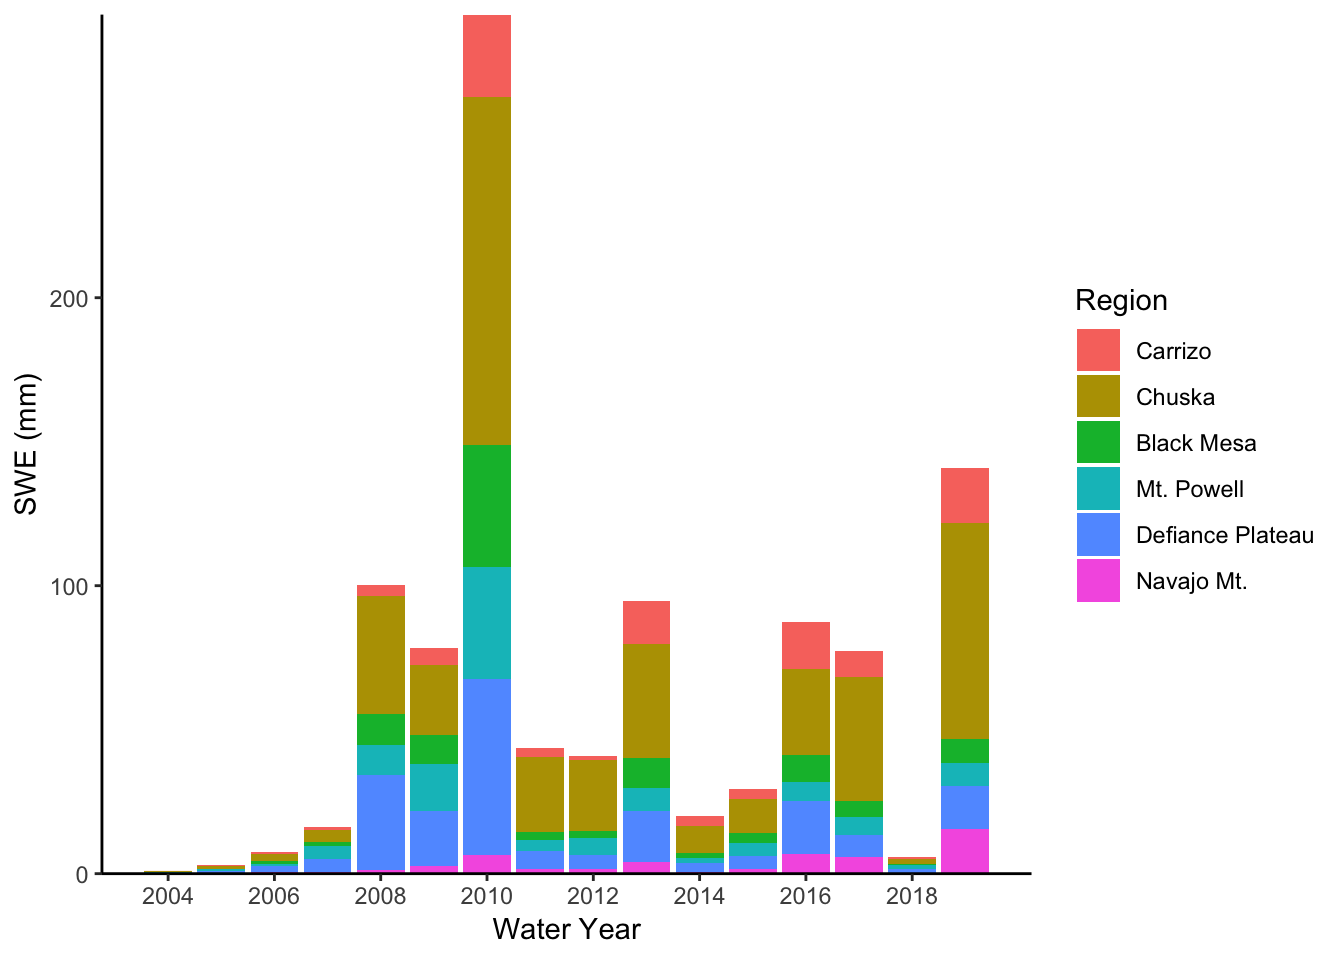
\includegraphics{SWE_final_analyses_files/figure-latex/unnamed-chunk-5-1.pdf}

\hypertarget{correlations-of-monthly-means-among-regions}{%
\subsubsection{Correlations of Monthly Means Among
Regions}\label{correlations-of-monthly-means-among-regions}}

Chuska vs Black Mesa R squared: 0.5590291

Chuska vs Carrizo R squared: 0.7066451

Black Mesa vs Carrizo R squared: 0.7516408

\hypertarget{appendix}{%
\subsection{Appendix}\label{appendix}}

Just to view these a bit better:

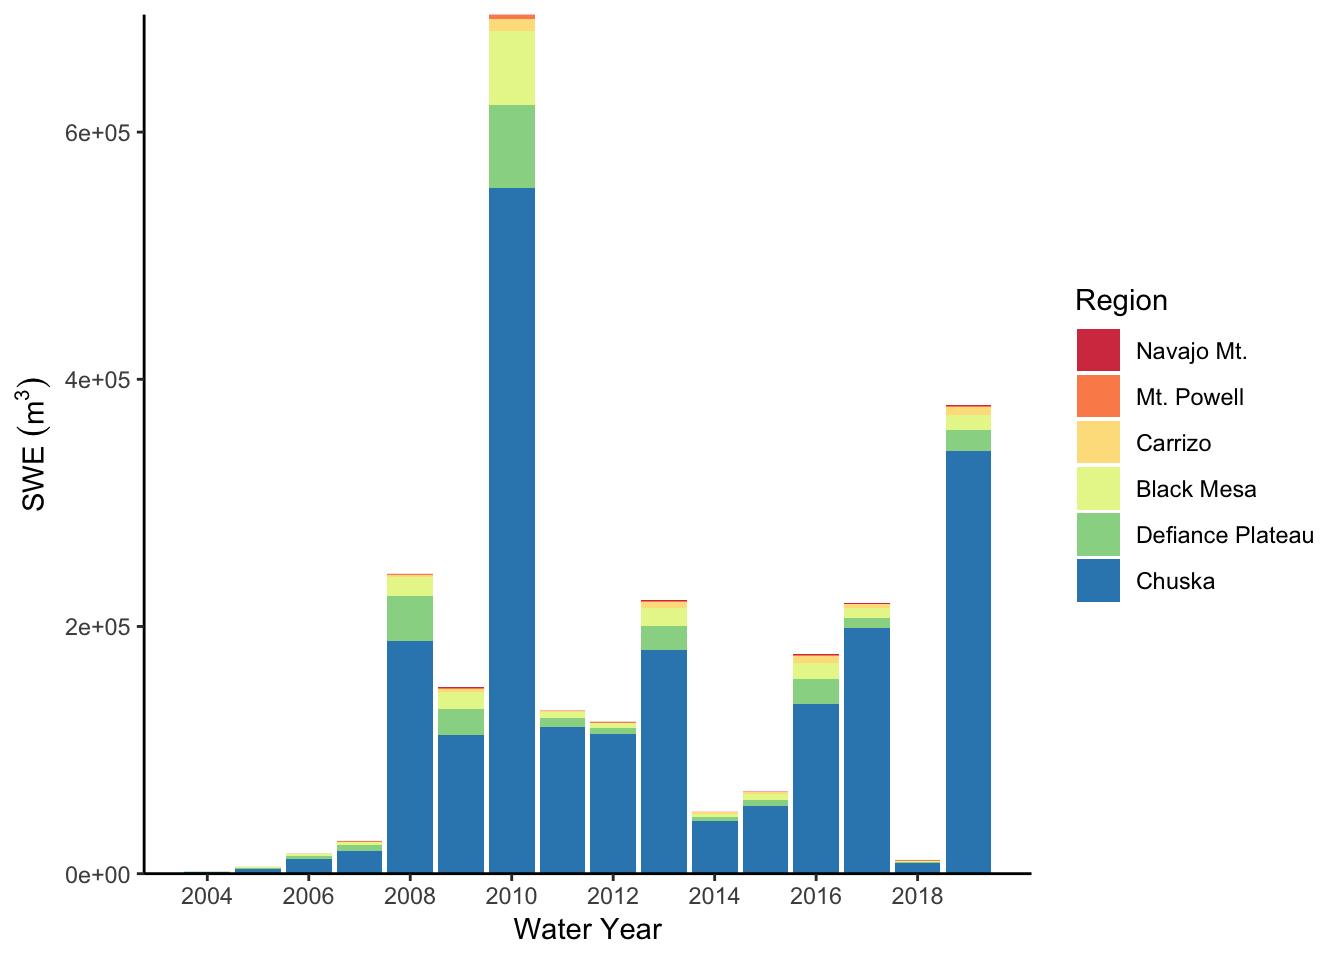
\includegraphics{SWE_final_analyses_files/figure-latex/unnamed-chunk-7-1.pdf}
\includegraphics{SWE_final_analyses_files/figure-latex/unnamed-chunk-7-2.pdf}
\includegraphics{SWE_final_analyses_files/figure-latex/unnamed-chunk-7-3.pdf}


\end{document}
